In een circuit moet wat erin gaat er ook uit komen. Als in een formule 1 wedstrijd 18 auto's aan de start verschijnen, dan zou het fijn zijn als er ook 18 auto's aan de finish komen. Mist er een auto dan is er wat fout gegaan. Als in een elektronisch circuit er aan het einde niet meer dezelfde hoeveelheid stroom is als aan het begin dan spreken we van een lek. Lekstromen kunnen gevaarlijk zijn, want het kan betekenen dat een deel van de stroom via een mens een andere route gevonden heeft. Om de mens te beschermen tegen deze stroom is er de aardlekschakelaar\index{Aardlekschakelaar}\index{Earth Leakage Circuit Breaker}. Als de elektronica in de schakelaar detecteerd dat er stroom "verdwenen" is dan schakelt de schakelaar het circuit uit.

In de elektronica wordt een aardlekschakelaar weergegeven met het symbool dat je ziet weergegeven in \ref{symbool:aardlekschakelaar}

\begin{figure}[h]
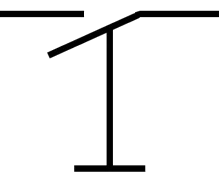
\includegraphics[width=5cm]{aardlekschakelaar}
\centering
\caption{Symbool van een aardlekschakelaar}
\label{symbool:aardlekschakelaar}
\end{figure}

